%!TEX root = ../main.tex

\section{Intervallschätzer - Konfidenzintervalle}
Die Intervallschätzer geben ein Intervall an, in dem sich der zu schätzende Parameter höchstwahrscheinlich befindet. Hierbei sind möglichst kleine Intervalle bei einer hohen Sicherheit natürlich gewünscht, aber diese Einschränkungen widersprechen sich. 
Verkleinert man das Intervall wird die Sicherheit, dass der geschätze Parameter wirklich enthalten ist im Allgemeinen kleiner.

Wir möchten nun zum Beispiel herausfinden, wie sicher wir uns sind, dass das Ergebnis eines Punktschätzers stimmt. Dafür bestimmen wir das \emph{Vertrauens- bzw. Konfidenzintervall}
\begin{equation*}
	J_n\coloneqq [\theta_u\circ X,\theta_o\circ X]
\end{equation*}
wobei wir den Parameter $\theta$ schätzen, der Werte aus $\Theta$ annimmt. Die Zufallsvariablen 
\begin{equation*}
	\theta_u\circ X,\theta_o\circ X: \Omega\rightarrow \Theta 
\end{equation*}
stellen dabei die untere und die obere Intervallgrenze dar (sinnvollerweise soll also $\theta_u\circ X\leq \theta_o\circ X$ gelten). Sie beschreiben einen Grenzwert von $\theta$ in Abhängigkeit von der Stichprobe.

Dieses Intervall $J_n$ soll das unbekannte $\theta$ mit einer \emph{Garantiewahrscheinlichkeit} von $(1-\alpha)$ enthalten, das heißt
\begin{equation}\label{eq:intervall}
	P_\theta (\theta\in J_n)=P_\theta(\theta_u\circ X\leq \theta\leq \theta_o\circ X)\geq 1-\alpha
\end{equation}
für alle Werte des Parameters $\theta$.


\subsection{Abschätzen mit der Tschebyscheff-Ungleichung}
Eine grobe Abschätzung dieser Grenzen kann zum Beispiel über die \hyperref[tschebyscheff]{Tschebyscheff-Ungleichung} erfolgen.
Damit kann man die Wahrscheinlichkeit, dass der Parameter außerhalb des Intervalls liegt
\begin{equation*}
	P_\theta(|X-\theta|\geq \epsilon)\leq \frac{V(X)}{\epsilon^2}= \alpha
\end{equation*}
beschränken.
Es ergibt sich mit der Umformung 
\begin{equation*}
	\frac{V(X)}{\epsilon^2}= \alpha \quad \Leftrightarrow \quad \epsilon =\sqrt{\frac{V(X)}{\alpha}}
\end{equation*}
die Abschätzung für die beiden Intervallgrenzen
\begin{align*}
	\theta_u(X)&=X-\sqrt{\frac{V(X)}{\alpha}}\\
	\theta_o(X)&=X+\sqrt{\frac{V(X)}{\alpha}}.
\end{align*}
Diese garantiert für alle $\theta\in\Theta$, dass der unbekannte Parameter $\theta$ nur mit Unsicherheit $\alpha$ außerhalb des geschätzten Intervalls liegt.
\begin{equation*}
	P_\theta(\theta\not\in J_n)=\textstyle P_\theta\left(\theta\not\in \left[ X-\sqrt{\frac{V(X)}{\alpha}},X+\sqrt{\frac{V(X)}{\alpha}}\right]\right)\leq \alpha.
\end{equation*}



\subsection{Abschätzen über die Verteilungsfunktion}
Die Ergebnisse, die man durch die Abschätzung mit Tschebyscheff erhält, sind sehr grob. Einen genaueren Ansatz bietet die Abschätzung der Intervallgrenzen über die Verteilungsfunktion.

Wir wollen die Wahrscheinlichkeit eines Ereignisses mit der Garantiewahrscheinlichkeit beschränken, siehe \autoref{eq:intervall}. Dieses vom Parameter $\theta$ abhängige Ereignis ist
\begin{equation*}
	A_\theta = \simpleset{\theta_u\circ X\leq \theta\leq \theta_o\circ X} = \simpleset{\theta\in J_n}
\end{equation*}
Um die beiden Schranken mit der Verteilungsfunktion abzuschätzen, betrachten wir das Komplement dieses Ereignisses
\begin{equation*}
	\overline A_\theta =\simpleset{\theta_u\circ X > \theta}+\simpleset{\theta_o\circ X< \theta}.
\end{equation*}
Die Wahrscheinlichkeit dieses Ereignisses soll durch die Unsicherheit beschränkt sein
\begin{equation*}
	P_\theta(\overline A_\theta) = P_\theta(\theta_u\circ X > \theta)+P_\theta(\theta_o\circ X< \theta)\overset!\leq\alpha
\end{equation*}
Man sieht, dass dies durch Abschätzen der beiden Teile mit $\beta=\frac\alpha2$ erreicht werden kann
\begin{align}
	P_\theta(\theta_u\circ X > \theta)\overset!\leq \beta \label{eq:untereSchranke}\\
	P_\theta(\theta_o\circ X< \theta)\overset!\leq\beta \label{eq:obereSchranke}
\end{align}
Wir bestimmen die Schranken $\theta_u(k)$ und $\theta_o(k)$ so, dass die folgenden beiden Gleichungen gelten. Diese implizieren dann die Forderung.
\begin{align*}
	P_{\theta_u(k)}(X\geq k)\overset!=\beta\quad\Rightarrow (\ref{eq:untereSchranke})\\
	P_{\theta_o(k)}(X\leq k)\overset!=\beta\quad\Rightarrow (\ref{eq:obereSchranke})
\end{align*}

\paragraph{Beispiel:}
Ein kleines Beispiel, bei dem wir die Intervallgrenzen in Abhängigkeit von $\beta$ bestimmen werden.
Ist $X\sim\binomial(2,p)$, dann betrachten wir zunächst die Funktion
\begin{equation*}
	P_p(X=k)=\binom *2k p^k(1-p)^{2-k}=\begin{cases}
		(1-p)^2,&k=0\\
		2*p(1-p),&k=1\\
		p^2,&k=2
	\end{cases}
\end{equation*}
Möchten wir nun die Intervallgrenzen $p_u(k)$ beziehungsweise $p_o(k)$ bestimmen ergeben sich wie oben die folgenden Gleichungen
\begin{align*}
	P_{p_o(0)}(X\leq 0)&=(1-p_o(0))^2\overset!=\beta&\Rightarrow p_o(0)&=1-\sqrt\beta\\
	P_{p_o(1)}(X\leq 1)&=(1-p_o(1))^2+2p_o(1)*(1-p_o(1))\overset!= \beta &\Rightarrow p_o(1)&=\sqrt{1-\beta}\\
	P_{p_u(1)}(X<1)&=(1-p_u(1))^2\overset!=1-\beta&\Rightarrow p_u(1)&=1-\sqrt{1-\beta}\\
	P_{p_u(2)}(X<2)&=(1-p_u(2))^2+2p_u(2)*(1-p_u(2))\overset!=1-\beta &\Rightarrow p_u(2)&=\sqrt{\beta}\\
\end{align*}

\subsection{Approximation über die Normalverteilung}
Für große $n$ werden Binomialverteilungen und das Schätzen von $p$ in der Praxis oft auf die Normalverteilung zurückgeführt und das Problem auf eine Quantilsbestimmung reduziert.
Denn es gilt nach dem zentralen Grenzwertsatz für $S_n\sim\binomial(n,p)$ und große $n$
\begin{equation*}
	P_p(S_n\leq k) = F^{S_n}_p(k)\overset{\text{ZGWS}}\approx \Phi\left(\frac{k-np+\frac12}{\sqrt{np(1-p)}}\right).
\end{equation*}
Hierbei ist die Korrektur um $\frac12$ eine sogenannte Stetigkeitskorrektur.

Damit lassen sich dann die Intervallgrenzen $p_u,p_o$ mit den Quantilen der Standardnormalverteilung bestimmen. Natürlich sind $n,k$ sowie $\beta$ bekannt.
\begin{align*}
	P_{p_o}(S_n\leq k)\approx \Phi\left(\frac{k-np_o+\frac12}{\sqrt{n*p_o(1-p_o)}}\right)&\overset!=\beta
	&\Rightarrow \frac{k-np_o+\frac12}{\sqrt{n*p_o(1-p_o)}}&=z_\beta\\
	P_{p_u}(S_n\geq k)=1-P_{p_u}(S_n<k)\approx 1-\Phi\left(\frac{k-np_u+\frac12}{\sqrt{n*p_u(1-p_u)}}\right)&\overset!=\beta
	&\Rightarrow \frac{k-np_u+\frac12}{\sqrt{n*p_u(1-p_u)}}&=z_{1-\beta}=-z_\beta\\
\end{align*}
Diese Gleichungen muss man nur noch nach $p_u$ bzw. $p_o$ auflösen (eventuell mit der Mitternachtsformel) und man erhält die Intervallgrenzen zur gegebenen Unsicherheit $\alpha=2\beta$.

\begin{center}
	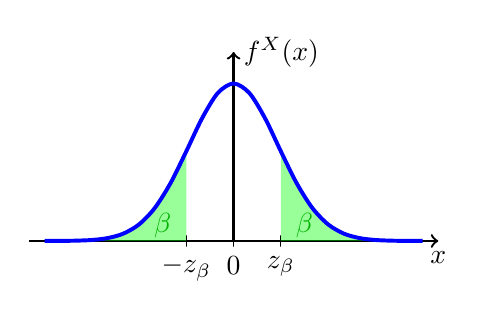
\begin{tikzpicture}[scale=0.4]
		\draw[->, line width=0.3mm] (-6.5,0) to (6.5,0) node[below] {$x$};
		\draw[->, line width=0.3mm] (0,0) to (0,6) node[right] {$f^X(x)$};

		\filldraw[scale=1,domain=-6:-1.5,smooth,variable=\x,fill=green, opacity=0.4, draw=none] plot ({\x},{5*exp(-\x*\x/4)}) -- (-1.5,0);
		\filldraw[scale=1,domain=1.5:6,smooth,variable=\x,fill=green, opacity=0.4, draw=none] plot ({\x},{5*exp(-\x*\x/4)}) -- (1.5,0);
		
		\draw[line width=0.5mm,scale=1,domain=-6:6,smooth,variable=\x,blue] plot ({\x},{5*exp(-\x*\x/4)});

		\draw (1.5,0) node (zp) [rectangle,inner sep = 0pt,minimum size = 0pt,minimum height=4pt,draw, label={below:$z_\beta$}] {};
		\draw (-1.5,0) node (-zp) [rectangle,inner sep = 0pt,minimum size = 0pt,minimum height=4pt,draw, label={below:$-z_{\beta}$}] {};

		\draw (-2.25,0.5) node[green!70!black] {$\beta$};
		\draw (2.25,0.5) node[green!70!black] {$\beta$};
		
		\draw (0,0) node (null) [rectangle,inner sep = 0pt,minimum size = 0pt,minimum height=4pt,draw, label={below:$0$}] {};
		
	\end{tikzpicture}	
\end{center}

\paragraph{Beispiel:}
Sei $X\sim\binomial(n=50,p)$ und es liegt eine Stichprobe mit $k=X(\omega)=30$ vor. Wir möchten nun zur Unsicherheit $\alpha=2\beta=0.05$, d.h. mit $90\%$-iger Sicherheit angeben, in welchem Intervall sich $p$ befindet.

Wir verwenden wieder die Gleichungen von oben und möchten die Intervallgrenzen $p_u,p_o$ bestimmen
\begin{align*}
	P_{p_o}(X\leq 30)\approx\Phi\left(\frac{30-50p_o+\frac12}{\sqrt{50p_o*(1-p_o)}}\right)&\overset!=\beta=0.05\\
	P_{p_u}(X< 30)&\overset!=1-\beta=0.95
\end{align*}
Wir bestimmen also das $\beta$ sowie das $1-\beta$-Quantil
\begin{align*}
	\Phi(-1.6449)&=0.05\\
	\Phi(1.6449)&=0.95
\end{align*}
Dies können wir dann in folgende Formel einsetzen. Da es sich jeweils um $\pm z_\beta$ handelt, muss die Formel nur einmal ausgerechnet werden, denn $z_\beta$ wird quadriert und wir finden beide Lösungen.
\begin{align*}
	\frac{k-np+\frac12}{\sqrt{np(1-p)}}&=\pm z_\beta\\
	\Leftrightarrow\enspace (n^2-z_\beta^2n)p^2+(-2nk-z_\beta^2n)p+k^2+\frac14&=0.\\
	\intertext{Mit den eingesetzten Werten erhält man schließlich}
	\frac{30-50*p+\frac12}{\sqrt{50p(1-p)}}&=\pm 1.6449\\
	\overset{\text{MNF}}\Rightarrow p_u=0.42049,\ & p_o=0.90537.
\end{align*}
